\section{Theorie}
\label{sec:Theorie}

Zwei über eine Kopplung verbundene Schwingsysteme werden gekoppelte Systeme genannt.
Wird eines der Systeme ausgelenkt, während das andere ruht, findet aufgrund der Kopplung ein Energieübertrag statt. Das ausgelenkte Systeme schwingt mit immer kleinerer Amplitude, bis es zum Stehen kommt, während 
das zunächst ruhende System mit immer größerer Amplitude schwingt. Dabei schwingt jedes System mit seiner Eigenfrequenz. Werden Energieverluste vernachlässigt, wiederholt sich dieser Vorgang immer wieder.

Im Folgenden werden zwei über einen Kopplungskondensator gekoppelte elekrische Schwingkreise betrachtet. Ein schematischer Aufbau des gekoppelten System ist in \autoref{fig:gekoppSchwingkreis} zu sehen.

\begin{figure}[H]
    \centering
    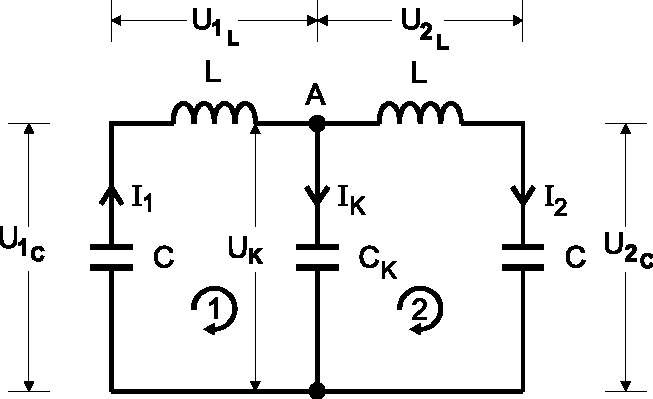
\includegraphics{SchwingkreisAbb.pdf}
    \caption{Schematische Darstellung eines gekoppelten Schwingkreises\cite{ap04}.}
    \label{fig:gekoppSchwingkreis}
\end{figure}

\newpage

Mithilfe der Kirchhoffschen Knoten- und Maschenregel ergeben sich

\begin{align*}
    I_k &= I_1-I_2\, ,\\
    0   &= U_{1,C} + U_{1,L} + U_K\, , \\ 
    0   &= U_{2,C} + U_{2,L} + U_K\,.
\end{align*}

Mit 
\begin{equation*}
    U_C = \dfrac{1}{C} \int I \, \text{d}t
\end{equation*}
und
\begin{equation*}
    U_L = L \dot{I}
\end{equation*}
ergeben sich nach Differenzieren nach der Zeit
\begin{equation}
    L\ddot{I}_1 + \dfrac{1}{C}I_1 + \dfrac{1}{C_k}(I_1 - I_2) = 0
    \label{eq:DGL1}
\end{equation}
und
\begin{equation}
    L\ddot{I}_2 + \dfrac{1}{C}I_2 - \dfrac{1}{C_k}(I_1 - I_2) = 0\,.
    \label{eq:DGL2}
\end{equation}

Werden nun \eqref{eq:DGL1} und \eqref{eq:DGL2} addiert bzw. subtrahiert, entstehen zwei lineare Differentialgleichungen mit den Variablen $I_1+I_2$ bzw. $I_1-I_2$.
Es folgen
\begin{equation}
    L \,\diff{^2}{t^2}(I_1+I_2) + \dfrac{1}{C}(I_1 + I_2) = 0
    \label{eq:addDGL}
\end{equation}
und
\begin{equation}
    L \,\diff{^2}{t^2}(I_1 - I_2) + \left(\dfrac{1}{C} + \dfrac{2}{C_k} \right)(I_1 - I_2) = 0\,.
\end{equation}

\newpage

Als homogene Differentialgleichungen des harmonischen Oszillators sind die Lösungen gegeben durch

\begin{equation}
    (I_1+I_2)(t) = I_{0,+} \cos(ω_+t)
    \label{eq:gleiSchwi}
\end{equation}
mit 
\begin{align*}
    I_{0,+} &= I_{1,0}+I_{2,0}\, , \\
    ω_+     &=\dfrac{1}{\sqrt{LC}}
\end{align*}
sowie

\begin{equation*}
    (I_1-I_2)(t) = I_{0,-}\cos(ω_-t)
    \label{eq:gegSchwi}
\end{equation*}
mit 
\begin{align*}
    I_{0,-} &=I_{1,0} - I_{2,0}\, , \\
    ω_-     &= \dfrac{1}{\sqrt{L \left(\dfrac{1}{C}+\dfrac{2}{C_k}\right)^{-1}}}\,.
\end{align*} \\

Aus \eqref{eq:gleiSchwi} und \eqref{eq:gegSchwi} lassen sich nun Lösungen für $I_1(t)$ und $I_2(t)$ bestimmen, die sich zu
\begin{equation}
    I_1(t) = \dfrac{1}{2}(I_{0,+}\cos(ω_+ t) + I_{0,-}\cos(ω_- t))
\end{equation}
und
\begin{equation}
    I_2(t) = \dfrac{1}{2}(I_{0,+}\cos(ω_+ t) - I_{0,-}\cos(ω_- t))
\end{equation}
ergeben. \\

Ist nun $I_{1,0} = I_{2,0}$, ist auch $I_{0,-} = 0$, $I_1(t)$ und $I_2(t)$ schwingen zu jedem Zeitpunkt $t$ mit der Frequenz $ν_+ = \dfrac{1}{2πω_+}$ in Phase und es gilt
\begin{equation*}
     I_1(t) = I_2(t) = I_0 \cos(ω_+ t)\,.
\end{equation*}

Analog ergibt sich für eine gegenphasige Schwingung, also $I_{1,0} = -I_{2,0}$, $I_{0,+}=0$ und damit
\begin{equation*}
    I_1(t) = I_0 \cos(ω_- t) = -I_2(t)\,.
\end{equation*}
Dabei schwingt das System mit der erhöhten Frequenz $ν_- = \dfrac{1}{2πω_-}$. Die gleich- und gegenphasigen Schwingungen des gekoppelten Systems werden als Fundamentalschwingungen bezeichnet.

Es lässt sich ein weiterer Spezialfall beobachten. Wird eine der beiden Startamplituden, hier $I_{2,0}$, auf null gesetzt, während die andere verschieden von null ist, stellt sich eine gekoppelte Schwingung ein.
Die Stromverläufe ergeben sich dann zu
\begin{equation}
    I_1(t) = \dfrac{1}{2} I_{1,0}(\cos(ω_+ t) + \cos(ω_- t))
    \label{eq:gekoSchwi1}
\end{equation}
und
\begin{equation}
    I_2(t) = \dfrac{1}{2} I_{1,0}(\cos(ω_+ t) - \cos(ω_- t))\,.
    \label{eq:gekoSchwi2}
\end{equation}

Unter Anwendung von
\begin{equation*}
    \cos(a) + \cos(b) = 2 \cos(\dfrac{1}{2}(a+b)) \cos(\dfrac{1}{2}(a-b))
\end{equation*} 

\begin{equation*}
    \cos(a) - \cos(b) = 2 \sin(\dfrac{1}{2}(a+b)) \sin(\dfrac{1}{2}(a-b))
\end{equation*} 

lassen sich \eqref{eq:gekoSchwi1} und \eqref{eq:gekoSchwi2} zu
\begin{equation*}
    I_1(t) = I_{1,0}\cos(\dfrac{1}{2}(ω_+ + ω_-)t) \cos(\dfrac{1}{2}(ω_+ - ω_-)t) 
\end{equation*}
und
\begin{equation*}
    I_2(t) = I_{1,0}\sin(\dfrac{1}{2}(ω_+ + ω_-)t) \sin(\dfrac{1}{2}(ω_+ - ω_-)t)
\end{equation*}
vereinfachen.
